\documentclass[border=3pt]{standalone}
\usepackage{tikz}
\usetikzlibrary{arrows.meta,calc}
\begin{document}
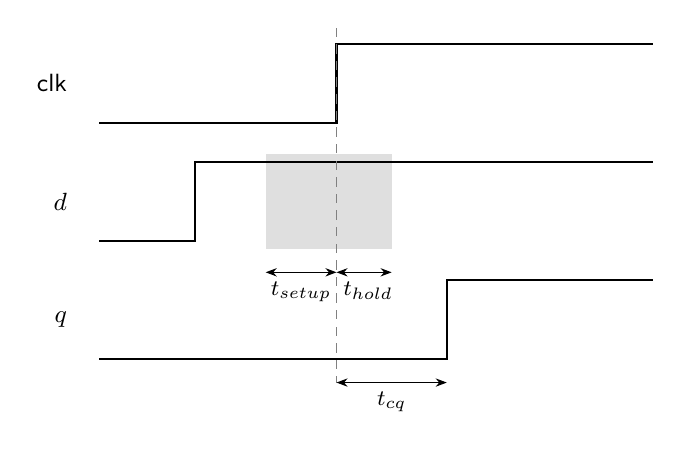
\begin{tikzpicture}[font=\sffamily\small, line cap=rect]
  % clk with rising edge at x=3
  \node[left] at (-0.3,0.5) {clk};
  \draw[thick] (0,0) -- (3,0) -- (3,1) -- (7,1);
  % aperture window around the edge
  \fill[gray!25] (2.1,-1.6) rectangle (3.7,-0.4);
  % d: must be stable inside the window; changes at 1.2
  \node[left] at (-0.3,-1.0) {$d$};
  \draw[thick] (0,-1.5) -- (1.2,-1.5) -- (1.2,-0.5) -- (7,-0.5);
  % q: changes t_cq after the edge
  \node[left] at (-0.3,-2.5) {$q$};
  \draw[thick] (0,-3) -- (4.4,-3) -- (4.4,-2) -- (7,-2);
  % edge marker
  \draw[dashed, gray] (3,1.2) -- (3,-3.3);
  % timing arrows
  \draw[{Stealth[length=4pt]}-{Stealth[length=4pt]}] (2.1,-1.9) -- (3,-1.9);
  \node[below, font=\footnotesize] at (2.55,-1.9) {$t_{setup}$};
  \draw[{Stealth[length=4pt]}-{Stealth[length=4pt]}] (3,-1.9) -- (3.7,-1.9);
  \node[below, font=\footnotesize] at (3.4,-1.9) {$t_{hold}$};
  \draw[{Stealth[length=4pt]}-{Stealth[length=4pt]}] (3,-3.3) -- (4.4,-3.3);
  \node[below, font=\footnotesize] at (3.7,-3.3) {$t_{cq}$};
\end{tikzpicture}
\end{document}
